% !TEX root = ../main.tex
% File: chapters_part1/chap4_1.tex
% Nội dung cho Chương 4, Phần 1

\section{Kiến trúc Transformer Gốc ("Attention Is All You Need")}
\label{sec:vanilla_transformer}

Để hiểu được sức mạnh của Transformer, chúng ta cần mổ xẻ từng khối xây dựng nên nó, bắt đầu từ ý tưởng cốt lõi nhất: Self-Attention.

\subsection{Chi tiết cơ chế Self-Attention: Scaled Dot-Product và Multi-Head Attention}
\label{ssec:self_attention}

Cơ chế chú ý mà chúng ta đã học trong mô hình Seq2Seq (ở mục \ref{sec:seq2seq_attention}) là \textit{cross-attention}, nơi Decoder "chú ý" đến Encoder. \textbf{Self-Attention (Tự chú ý)} là một biến thể đặc biệt, nơi một chuỗi "chú ý" đến chính nó.

\paragraph{Tư duy cốt lõi}
Self-Attention cho phép mỗi từ trong một câu có thể "nhìn" vào tất cả các từ khác trong cùng một câu để tính toán ra một biểu diễn mới cho chính nó. Biểu diễn mới này không chỉ chứa thông tin của bản thân từ đó, mà còn được "làm giàu" bởi ngữ cảnh từ các từ liên quan nhất.

Ví dụ, trong câu "Con mèo không muốn băng qua đường vì nó quá mệt", khi xử lý từ "nó", Self-Attention sẽ giúp mô hình xác định rằng "nó" có liên quan mật thiết đến "mèo" chứ không phải "đường", và tạo ra một biểu diễn cho "nó" mang nhiều thông tin của "mèo".

\subsubsection{Scaled Dot-Product Attention}
Đây là khối xây dựng cơ bản của Self-Attention trong Transformer. Nó hoạt động dựa trên ba khái niệm được lấy cảm hứng từ các hệ thống tìm kiếm thông tin: \textbf{Query, Key, và Value}.

\begin{tcolorbox}[
    title={Trực giác về Query, Key, Value},
    colback=yellow!10!white, colframe=yellow!50!black, fonttitle=\bfseries
]
Hãy tưởng tượng bạn đang tìm kiếm video trên YouTube.
\begin{itemize}
    \item \textbf{Query (Truy vấn):} Là cụm từ bạn gõ vào thanh tìm kiếm (ví dụ: "công thức nấu phở"). Nó đại diện cho \textit{thông tin bạn đang cần}.
    \item \textbf{Key (Khóa):} Mỗi video trên YouTube có một bộ các từ khóa (tiêu đề, mô tả) để mô tả nội dung của nó. Nó đại diện cho \textit{thông tin mà một đối tượng có thể cung cấp}.
    \item \textbf{Value (Giá trị):} Chính là nội dung của video. Nó đại diện cho \textit{thông tin thực sự sẽ được lấy ra}.
\end{itemize}
Cơ chế hoạt động là: bạn lấy \textbf{Query} của mình, so sánh nó với \textbf{Key} của tất cả các video để tìm ra các video liên quan nhất (tính điểm tương đồng). Sau đó, bạn lấy một "tổng có trọng số" của các \textbf{Value} (nội dung video), trong đó các video liên quan hơn sẽ có trọng số cao hơn.
\end{tcolorbox}

\begin{tcolorbox}[
    title={Tại sao lại cần đến ba vai trò Q, K, V?},
    colback=green!5!white, colframe=green!50!black, fonttitle=\bfseries
]
Một câu hỏi tự nhiên là: Tại sao mỗi từ đầu vào $x_i$ lại cần được chiếu thành ba vector $q_i, k_i, v_i$ riêng biệt? Tại sao không chỉ dùng chính các $x_i$?
\begin{itemize}
    \item \textbf{Sự linh hoạt:} Việc tách thành ba vai trò mang lại sự linh hoạt tối đa. Nó cho phép mô hình học cách so sánh các từ dựa trên một loại đặc trưng (được mã hóa trong $Q$ và $K$) và sau đó trích xuất một loại đặc trưng khác (được mã hóa trong $V$).
    \item \textbf{Ví dụ trực quan:} Hãy quay lại ví dụ "Con mèo... vì nó quá mệt".
        \begin{itemize}
            \item Khi tính toán biểu diễn cho "nó", \textbf{Query ($q_{\text{nó}}$)} có thể mã hóa thông tin: "Tôi là một đại từ, tôi cần tìm một danh từ làm tham chiếu".
            \item \textbf{Key ($k_{\text{mèo}}$)} của "mèo" có thể mã hóa: "Tôi là một danh từ giống đực/cái, số ít". Key này sẽ "khớp" rất tốt với Query của "nó".
            \item \textbf{Value ($v_{\text{mèo}}$)} của "mèo" có thể chứa thông tin ngữ nghĩa thực sự của từ: "một loài động vật bốn chân".
        \end{itemize}
        Sau khi $q_{\text{nó}}$ khớp với $k_{\text{mèo}}$, biểu diễn mới của "nó" sẽ nhận được một phần lớn thông tin từ $v_{\text{mèo}}$, giúp nó "hiểu" rằng nó đang nói về một con vật. Nếu chỉ dùng $x_i$ cho cả ba vai trò, mô hình sẽ bị hạn chế trong việc học các mối quan hệ phức tạp như vậy.
\end{itemize}
\end{tcolorbox}

Trong Self-Attention, mỗi từ đầu vào sẽ đóng cả ba vai trò này.
\paragraph{Cơ chế hoạt động chi tiết}
Giả sử chúng ta có một chuỗi các vector đầu vào $X = (x_1, x_2, \dots, x_n)$.
\begin{enumerate}
    \item \textbf{Tạo Query, Key, Value:} Chúng ta tạo ra ba ma trận trọng số có thể học được: $W^Q, W^K, W^V$. Mỗi vector đầu vào $x_i$ sẽ được nhân với ba ma trận này để tạo ra ba vector tương ứng:
        \begin{itemize}
            \item $q_i = W^Q x_i$ (Query vector của từ $i$)
            \item $k_i = W^K x_i$ (Key vector của từ $i$)
            \item $v_i = W^V x_i$ (Value vector của từ $i$)
        \end{itemize}
        Toàn bộ chuỗi sẽ tạo ra các ma trận $Q, K, V$.
    \item \textbf{Tính điểm chú ý (Attention Scores):} Để tính toán biểu diễn mới cho từ thứ $i$, chúng ta lấy Query của nó ($q_i$) và tính tích vô hướng (dot product) với Key của \textit{tất cả} các từ khác (bao gồm cả chính nó), $k_j$. Đây chính là bước so sánh "Query" với tất cả các "Key".
        $$ \text{score}(i, j) = q_i \cdot k_j $$
    \item \textbf{Chia tỷ lệ (Scaling):} Tích vô hướng có thể tạo ra các giá trị rất lớn, đẩy hàm softmax vào vùng có gradient rất nhỏ, gây khó khăn cho việc huấn luyện. Bài báo đã "scale" (chia) các điểm số này cho căn bậc hai của số chiều của vector Key, $d_k$.
        $$ \text{scaled\_score}(i, j) = \frac{q_i \cdot k_j}{\sqrt{d_k}} $$
    \item \textbf{Chuẩn hóa (Softmax):} Áp dụng hàm softmax trên các điểm số đã chia tỷ lệ để có được các trọng số chú ý $\alpha_{ij}$.
    \item \textbf{Tính toán đầu ra:} Biểu diễn đầu ra mới cho từ $i$, ký hiệu là $z_i$, được tính bằng tổng có trọng số của \textit{tất cả} các vector Value.
        $$ z_i = \sum_{j=1}^{n} \alpha_{ij} v_j $$
\end{enumerate}

Toàn bộ quá trình này có thể được tóm gọn trong một công thức ma trận duy nhất, cực kỳ hiệu quả cho việc tính toán trên GPU:
\begin{equation}
    \text{Attention}(Q, K, V) = \text{softmax}\left(\frac{QK^T}{\sqrt{d_k}}\right)V
    \label{eq:scaled_dot_product_attention}
\end{equation}

\begin{center}
    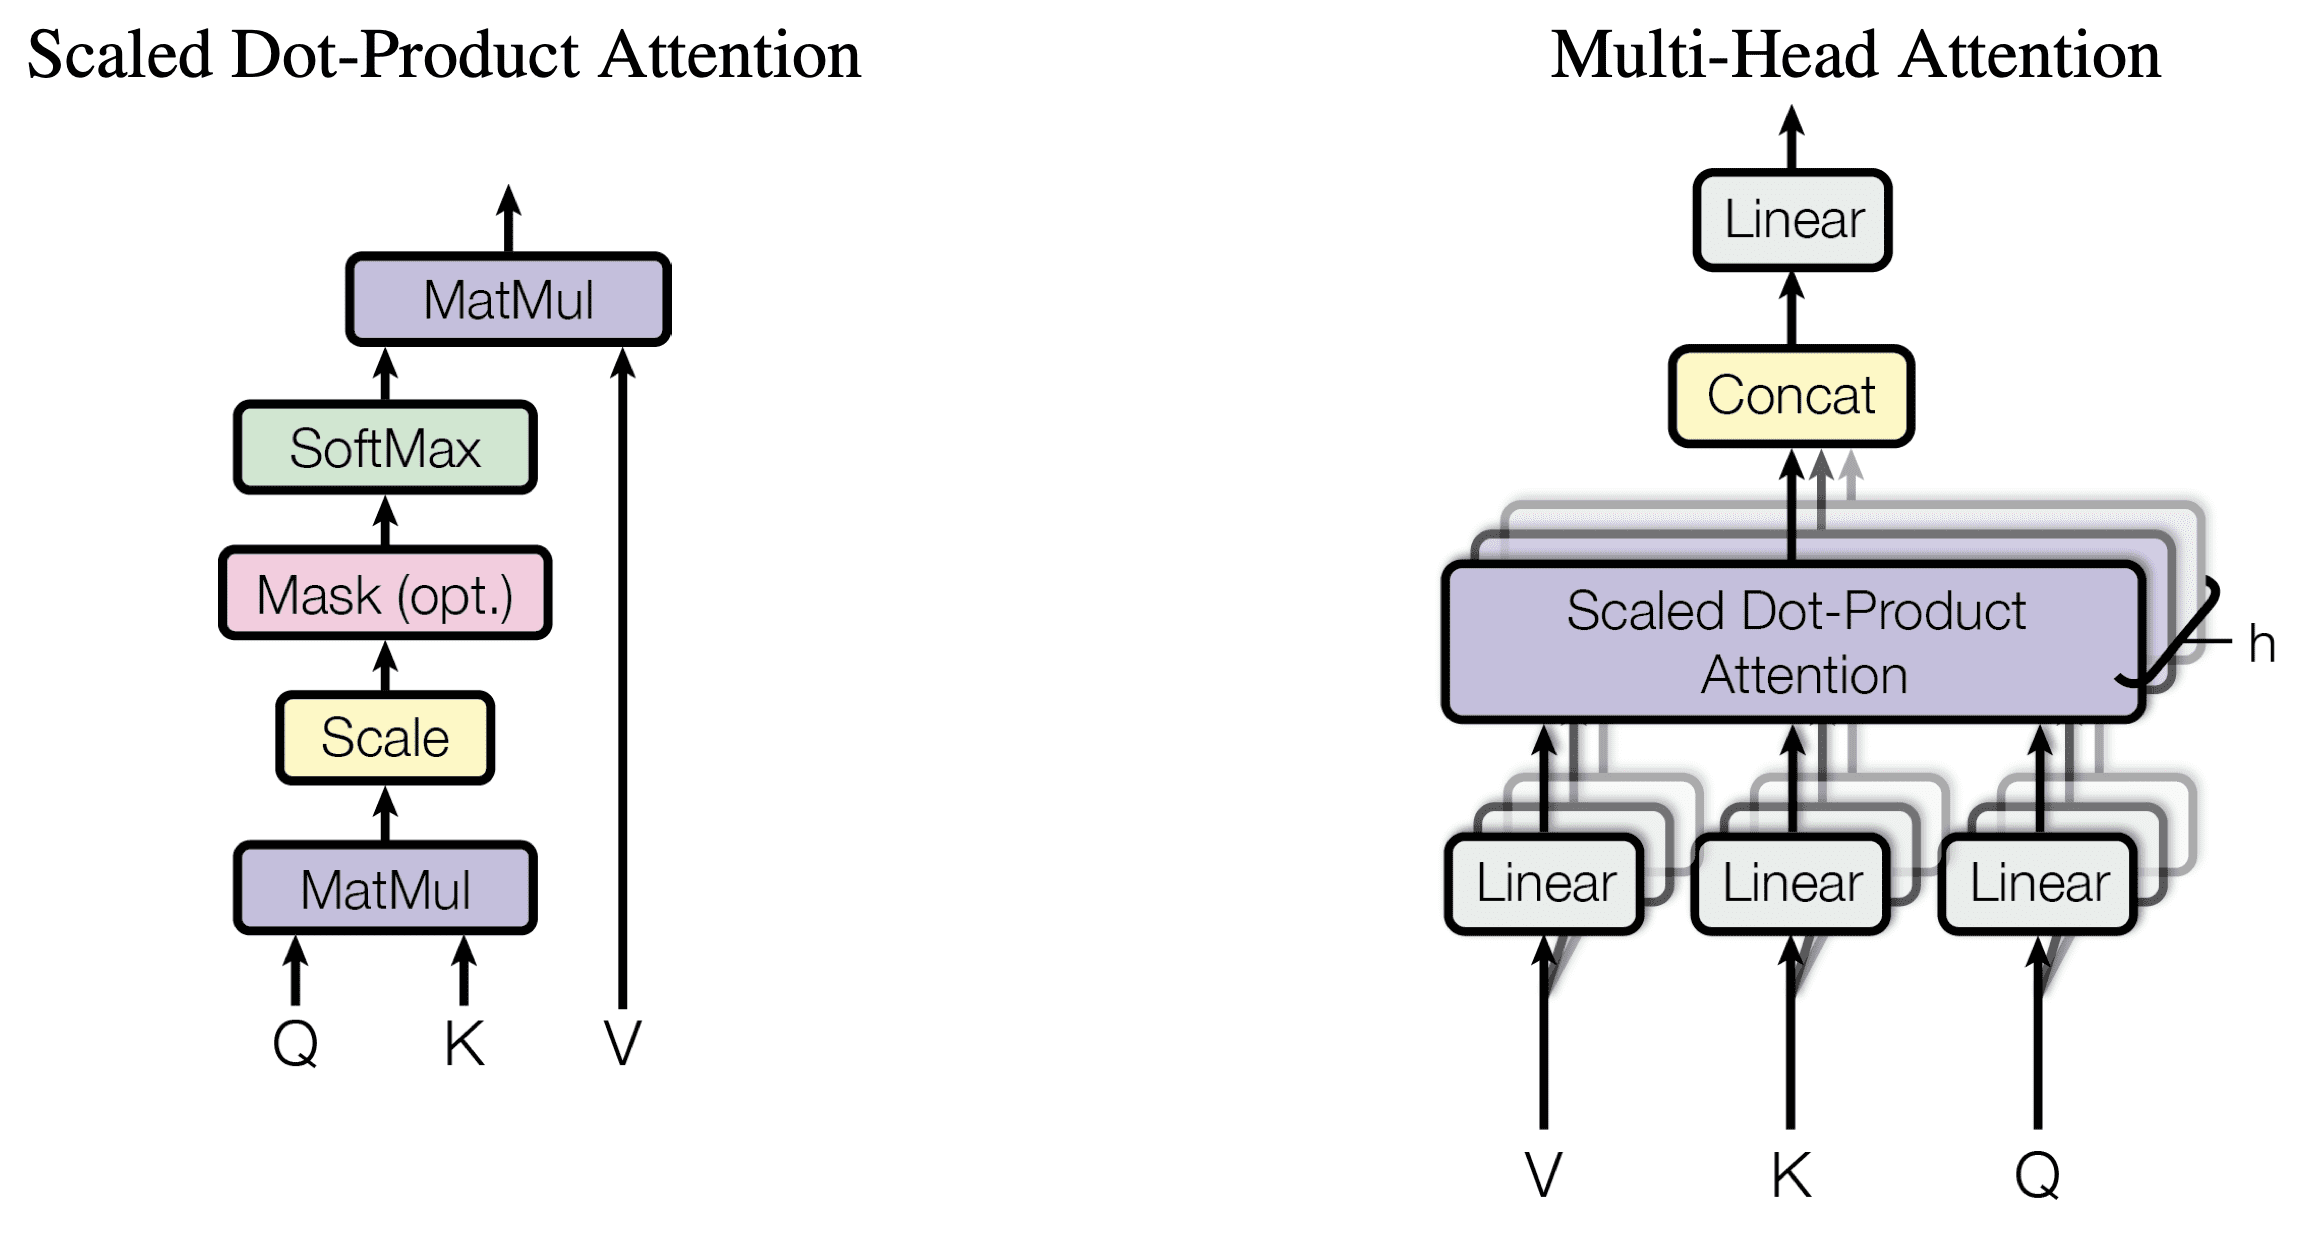
\includegraphics[width=0.6\textwidth]{scaled_dot_product_attention.png}
    \captionof{figure}{Sơ đồ Scaled Dot-Product Attention. Đầu vào là các ma trận Q, K, V và đầu ra là một ma trận đã được làm giàu ngữ cảnh.}
    \label{fig:scaled_dot_product_attention}
\end{center}

\subsubsection{Multi-Head Attention}
\paragraph{Vấn đề của Single-Head Attention}
Chỉ có một bộ Self-Attention duy nhất sẽ bị hạn chế. Nó giống như việc bạn chỉ có thể tập trung vào một khía cạnh của mối quan hệ giữa các từ. Ví dụ, khi xử lý câu "Con mèo ngồi trên chiếu", một "đầu" chú ý (attention head) có thể học cách liên kết "nó" với "mèo" (quan hệ đồng tham chiếu), nhưng có thể sẽ bỏ lỡ các mối quan hệ khác (ví dụ, quan hệ cú pháp).

\paragraph{Giải pháp: Nhiều "đầu" chú ý song song}
Multi-Head Attention giải quyết vấn đề này bằng cách chạy nhiều cơ chế Scaled Dot-Product Attention một cách \textbf{song song}.
\begin{itemize}
    \item Thay vì chỉ có một bộ trọng số $(W^Q, W^K, W^V)$, chúng ta có $h$ bộ (ví dụ, $h=8$).
    \item Mỗi bộ trọng số này $(W^Q_i, W^K_i, W^V_i)$ với $i=1,\dots,h$ được gọi là một "đầu" chú ý.
    \item Mỗi "đầu" sẽ chiếu các vector đầu vào vào một không gian con khác nhau và thực hiện Self-Attention một cách độc lập. Điều này cho phép mỗi đầu có thể học một loại quan hệ khác nhau. Ví dụ, một đầu có thể học quan hệ cú pháp, một đầu khác học quan hệ ngữ nghĩa, một đầu khác học quan hệ đồng tham chiếu...
    \item Các vector đầu ra từ tất cả các đầu sau đó được \textbf{nối lại (concatenated)} với nhau.
    \item Vector nối này sau đó được chiếu qua một ma trận trọng số cuối cùng $W^O$ để tạo ra vector đầu ra cuối cùng của lớp Multi-Head Attention.
\end{itemize}

\begin{center}
    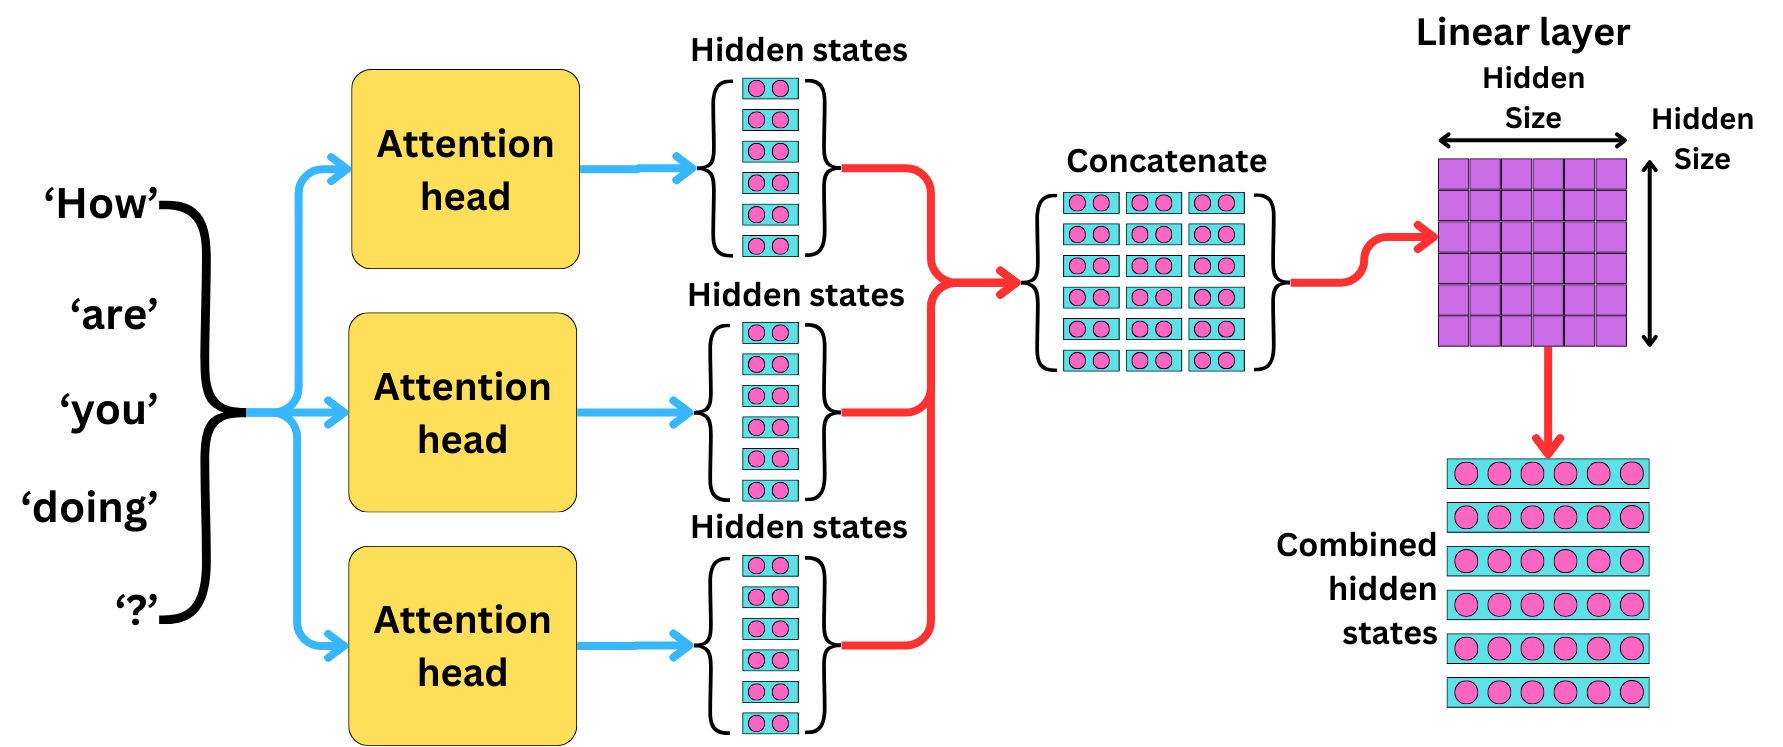
\includegraphics[width=0.8\textwidth]{multi_head_attention.png}
    \captionof{figure}{Kiến trúc Multi-Head Attention, bao gồm nhiều "đầu" Scaled Dot-Product Attention chạy song song.}
    \label{fig:multi_head_attention}
\end{center}

Multi-Head Attention cho phép mô hình cùng lúc chú ý đến thông tin từ các không gian biểu diễn khác nhau tại các vị trí khác nhau. Đây là một trong những nhân tố chính tạo nên sức mạnh biểu diễn của Transformer.

\subsection{Kiến trúc Encoder-Decoder và các thành phần phụ}
\label{ssec:transformer_architecture}
Transformer gốc vẫn giữ kiến trúc Encoder-Decoder của Seq2Seq, nhưng thay thế hoàn toàn các lớp RNN bằng các khối Self-Attention và các lớp Feed-Forward.

\subsubsection{The Encoder Stack}
Encoder của Transformer là một chuỗi gồm $N$ (ví dụ, $N=6$) khối Encoder giống hệt nhau được xếp chồng lên nhau. Mỗi khối bao gồm hai lớp con chính:
\begin{enumerate}
    \item \textbf{Multi-Head Self-Attention Layer:} Lớp này thực hiện Self-Attention trên chuỗi đầu vào.
    \item \textbf{Position-wise Feed-Forward Network (FFN):} Đây là một mạng nơ-ron truyền thẳng đơn giản, bao gồm hai lớp tuyến tính với một hàm kích hoạt ReLU ở giữa.
        $$ \text{FFN}(x) = \max(0, xW_1 + b_1)W_2 + b_2 $$
        FFN này được áp dụng một cách \textbf{độc lập và giống hệt nhau} cho từng vị trí (position) trong chuỗi.
\end{enumerate}
Ngoài ra, mỗi lớp con này còn được bao bọc bởi hai thành phần quan trọng khác:
\begin{itemize}
    \item \textbf{Residual Connection (Kết nối phần dư):} Đầu ra của mỗi lớp con là $\text{LayerNorm}(x + \text{Sublayer}(x))$. Tức là, đầu vào $x$ của lớp con được cộng trực tiếp vào đầu ra của chính lớp đó ($\text{Sublayer}(x)$). Kết nối phần dư này giúp gradient chảy dễ dàng hơn qua các mạng sâu và chống lại vấn đề triệt tiêu gradient.
    \item \textbf{Layer Normalization (Chuẩn hóa lớp):} Chuẩn hóa đầu ra của mỗi lớp con để ổn định quá trình huấn luyện.
\end{itemize}
\begin{tcolorbox}[
    title={Vai trò của các Thành phần Phụ trong Khối Transformer},
    colback=blue!5!white, colframe=blue!50!black, fonttitle=\bfseries
]
Nếu Self-Attention là "bộ não" thì FFN, Residual Connection và Layer Normalization là "hệ tuần hoàn và hệ thần kinh" giúp bộ não đó hoạt động ổn định và hiệu quả.
\begin{itemize}
    \item \textbf{Position-wise Feed-Forward Network (FFN):}
        \begin{itemize}
            \item \textbf{Vai trò:} Lớp Self-Attention chủ yếu thực hiện việc \textbf{trộn thông tin (mixing information)} giữa các từ. Sau bước này, lớp FFN được áp dụng riêng lẻ cho từng vị trí để \textbf{xử lý sâu hơn (deep processing)} thông tin đã được trộn đó. Nó có thể được xem như một bước "biến đổi phi tuyến" mạnh mẽ, giúp mô hình học các mối quan hệ phức tạp hơn, hoặc thậm chí hoạt động như một bộ nhớ key-value đơn giản để lưu trữ các tri thức đã học.
            \item \textbf{Tại sao "Position-wise"?} Việc áp dụng cùng một FFN cho mọi vị trí tương tự như việc chia sẻ trọng số trong RNN hoặc phép tích chập 1x1 trong CNN. Nó đảm bảo tính nhất quán trong cách xử lý ở các vị trí khác nhau.
        \end{itemize}
    \item \textbf{Residual Connection \& Layer Normalization:}
        \begin{itemize}
            \item \textbf{Mục đích kép của Residual Connection:} 1) Nó tạo ra một "con đường tắt" cho gradient, giúp chống lại vấn đề triệt tiêu gradient và cho phép huấn luyện các mô hình rất sâu (ví dụ, hàng chục lớp Transformer). 2) Nó đảm bảo rằng ngay cả khi một lớp con (Sublayer) không học được gì hữu ích, thông tin từ lớp trước đó vẫn có thể đi thẳng tới lớp tiếp theo mà không bị mất mát. Mô hình chỉ cần học phần "thay đổi" (delta) so với đầu vào.
            \item \textbf{Layer Normalization:} Nó giúp ổn định quá trình huấn luyện bằng cách giữ cho đầu ra của mỗi lớp con có phân phối ổn định (trung bình 0, phương sai 1). Điều này làm cho quá trình tối ưu hóa trở nên mượt mà hơn và ít nhạy cảm hơn với việc khởi tạo trọng số. Sự kết hợp của Residuals và Norm là công thức vàng để huấn luyện các mạng nơ-ron rất sâu thành công.
        \end{itemize}
\end{itemize}
\end{tcolorbox}
\subsubsection{The Decoder Stack}
Decoder cũng là một chuỗi gồm $N$ khối Decoder giống hệt nhau. Mỗi khối Decoder có ba lớp con:
\begin{enumerate}
    \item \textbf{Masked Multi-Head Self-Attention Layer:} Tương tự như Self-Attention của Encoder, nhưng có một sự thay đổi quan trọng: \textbf{masking (che giấu)}. Khi dự đoán từ ở vị trí $i$, Decoder chỉ được phép "chú ý" đến các từ ở các vị trí trước đó (từ $1$ đến $i$).
    \begin{itemize}
        \item \textbf{Cơ chế kỹ thuật:} Việc này được thực hiện bằng cách thêm một "ma trận mặt nạ" (mask matrix) vào ma trận điểm chú ý, ngay trước bước softmax. Ma trận này có giá trị là 0 cho các vị trí được phép chú ý và $-\infty$ cho các vị trí bị cấm.
        \item \textbf{Hệ quả:} Sau khi qua hàm softmax, các vị trí có giá trị $-\infty$ sẽ có trọng số chú ý bằng 0, đảm bảo rằng thông tin từ các từ tương lai không bị "rò rỉ" vào quá trình tính toán.
        \item \textbf{Mục đích:} Điều này là để đảm bảo tính \textbf{tự hồi quy (auto-regressive)} của mô hình, ngăn không cho nó "gian lận" bằng cách nhìn vào các từ mà nó đang cố gắng dự đoán. Nó mô phỏng quá trình sinh văn bản trong thực tế, nơi chúng ta chỉ biết những từ đã viết trước đó.
    \end{itemize}
    \item \textbf{Multi-Head Cross-Attention Layer:} Đây là nơi Decoder thực sự tương tác với Encoder, và là nơi kiến trúc "chú ý" của Seq2Seq gốc được tái hiện.
    \begin{itemize}
        \item \textbf{Dòng chảy thông tin:} Ở lớp này, \textbf{Query} được tạo ra từ đầu ra của lớp Masked Self-Attention của Decoder. Nó đại diện cho "câu hỏi" mà Decoder đang muốn hỏi: "Dựa trên những gì tôi đã dịch cho đến nay, tôi nên nhìn vào đâu trong câu gốc để dịch từ tiếp theo?".
        \item Trong khi đó, \textbf{Key và Value} được tạo ra từ \textbf{đầu ra của khối Encoder cuối cùng}. Chúng đại diện cho "kho thông tin" mà Decoder có thể truy vấn.
        \item \textbf{Kết quả:} Lớp này cho phép mỗi từ trong chuỗi đầu ra chú ý đến tất cả các từ trong chuỗi đầu vào, giúp mô hình căn chỉnh (align) các từ giữa hai ngôn ngữ một cách hiệu quả.
    \end{itemize}
    \item \textbf{Position-wise Feed-Forward Network:} Giống hệt như trong Encoder.
\end{enumerate}
Tương tự Encoder, mỗi lớp con của Decoder cũng có Residual Connection và Layer Normalization.

\subsubsection{Huấn luyện và Tối ưu hóa}
\label{sssec:transformer_training}
Kiến trúc Transformer gốc được huấn luyện cho tác vụ dịch máy. Tương tự như mô hình Seq2Seq, mục tiêu là tối thiểu hóa hàm mất mát \textbf{Cross-Entropy} giữa phân phối xác suất đầu ra của Decoder và từ tham chiếu (ground truth).

\begin{itemize}
    \item \textbf{Hàm Mất mát:} Lỗi được tính toán tại mỗi bước sinh từ của Decoder và được tổng hợp lại trên toàn bộ chuỗi.
    \item \textbf{Tối ưu hóa:} Bài báo gốc sử dụng bộ tối ưu hóa \textbf{Adam} \cite{kingma2014adam} với một lịch trình tốc độ học (learning rate schedule) đặc biệt bao gồm một giai đoạn "warmup" (tăng tuyến tính) sau đó là giảm dần theo hàm căn bậc hai nghịch đảo. Lịch trình này được chứng minh là rất quan trọng để huấn luyện Transformer một cách ổn định.
    \item \textbf{Điều chuẩn (Regularization):} Hai kỹ thuật điều chuẩn chính được sử dụng để tránh overfitting là \textbf{Dropout} \cite{srivastava2014dropout}, được áp dụng sau mỗi lớp con (trước kết nối phần dư), và \textbf{Label Smoothing}, một kỹ thuật làm cho các nhãn thật trở nên "mềm" hơn một chút (ví dụ, thay vì [0, 0, 1, 0], nhãn có thể là [0.025, 0.025, 0.9, 0.025]), giúp mô hình bớt tự tin thái quá và tổng quát hóa tốt hơn.
\end{itemize}

\subsection{Positional Encoding: Thêm thông tin về vị trí}
\label{ssec:positional_encoding_intro}

Một vấn đề lớn của việc loại bỏ RNN là chúng ta đã làm mất thông tin về \textbf{thứ tự của các từ}. Self-Attention, về bản chất, không nhạy cảm với vị trí; nếu ta hoán vị các từ trong câu, ma trận chú ý cũng sẽ bị hoán vị tương ứng mà không thay đổi bản chất.

Để giải quyết vấn đề này, Transformer thêm một vector gọi là \textbf{Positional Encoding (Mã hóa Vị trí)} vào các vector embedding đầu vào. Vector này cung cấp thông tin về vị trí tuyệt đối hoặc tương đối của một từ trong chuỗi.

\subsubsection{Absolute Positional Encoding (Sinusoidal)}
Đây là phương pháp được sử dụng trong bài báo gốc. Các vector mã hóa vị trí được tạo ra bằng các hàm sin và cos với các tần số khác nhau:
$$ PE_{(pos, 2i)} = \sin(pos / 10000^{2i/d_{\text{model}}}) $$
$$ PE_{(pos, 2i+1)} = \cos(pos / 10000^{2i/d_{\text{model}}}) $$
Trong đó $pos$ là vị trí của từ, $i$ là chỉ số chiều của vector, và $d_{\text{model}}$ là số chiều của embedding.
\paragraph{Tại sao lại dùng sin và cos?}
\begin{itemize}
    \item \textbf{Giá trị duy nhất:} Mỗi vị trí có một vector mã hóa duy nhất.
    \item \textbf{Mô hình có thể học quan hệ tương đối:} Có một tính chất toán học quan trọng: mã hóa vị trí của $pos+k$ có thể được biểu diễn như một hàm tuyến tính của mã hóa vị trí của $pos$. Điều này cho phép mô hình dễ dàng học cách chú ý đến các vị trí tương đối, ví dụ "từ cách 2 vị trí về bên phải".
    \item \textbf{Khả năng ngoại suy:} Có thể tạo ra vector mã hóa cho các chuỗi dài hơn những chuỗi đã thấy trong quá trình huấn luyện.
\end{itemize}

\subsubsection{Relative Positional Encoding}
Các phương pháp sau này cho rằng thông tin về khoảng cách tương đối ("từ này cách từ kia bao xa?") quan trọng hơn vị trí tuyệt đối. Các phương pháp mã hóa vị trí tương đối sẽ sửa đổi trực tiếp cơ chế Self-Attention, thêm một số hạng biểu diễn cho khoảng cách tương đối vào lúc tính điểm chú ý.

\subsubsection{Rotary Position Embedding (RoPE)}
Đây là một phương pháp mã hóa vị trí tương đối rất thanh lịch và hiệu quả \cite{su2021roformer}, được sử dụng trong nhiều LLM hiện đại như Llama.
\begin{itemize}
    \item \textbf{Ý tưởng:} Thay vì cộng, RoPE \textbf{xoay (rotates)} các vector Query và Key một góc phụ thuộc vào vị trí tuyệt đối của chúng.
    \item \textbf{Hệ quả:} Tích vô hướng giữa hai vector đã được xoay ($q_m^T k_n$) sẽ chỉ phụ thuộc vào vector ban đầu và \textbf{khoảng cách tương đối} giữa chúng ($m-n$), chứ không phụ thuộc vào vị trí tuyệt đối $m, n$.
\end{itemize}
RoPE đã chứng tỏ khả năng ngoại suy độ dài ngữ cảnh rất tốt và là một trong những phương pháp mã hóa vị trí hàng đầu hiện nay.